\documentclass[tikz,border=8pt]{standalone}
\usepackage{newtxtext,newtxmath}
\usetikzlibrary{arrows.meta}
\begin{document}
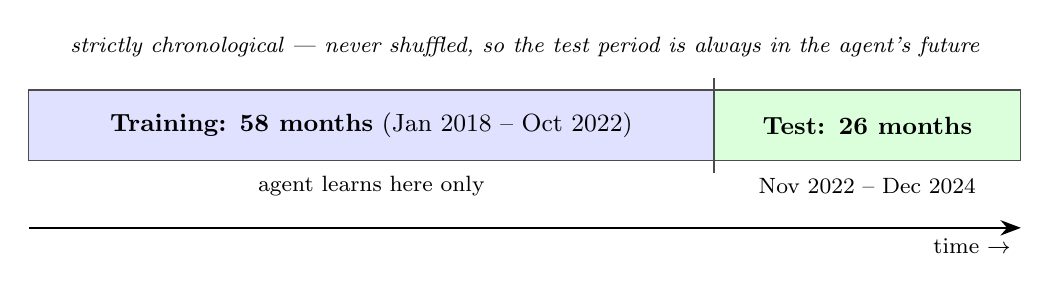
\begin{tikzpicture}[font=\small]
% timeline bar: 84 months, train 58 (69%), test 26 (31%)
\def\W{12.6} \def\H{0.9}
\def\SPLIT{8.7} % 58/84 of width
\draw[fill=blue!12, draw=black!70] (0,0) rectangle (\SPLIT,\H);
\draw[fill=green!14, draw=black!70] (\SPLIT,0) rectangle (\W,\H);
\node at (\SPLIT/2, \H/2) {\textbf{Training: 58 months} (Jan 2018 -- Oct 2022)};
\node at ({(\SPLIT+\W)/2}, \H/2) {\textbf{Test: 26 months}};
\node[font=\footnotesize] at ({(\SPLIT+\W)/2}, -0.32) {Nov 2022 -- Dec 2024};
\node[font=\footnotesize] at (\SPLIT/2, -0.32) {agent learns here only};
\draw[-{Stealth[length=2.6mm]}, thick] (0,-0.85) -- (\W,-0.85)
  node[pos=1, below left, font=\footnotesize]{time $\rightarrow$};
\draw[thick, black!70] (\SPLIT, -0.15) -- (\SPLIT, \H+0.15);
\node[font=\footnotesize\itshape, align=center] at (\W/2, \H+0.55)
  {strictly chronological --- never shuffled, so the test period is always
   in the agent's future};
\end{tikzpicture}
\end{document}
